The main components of a logic tree structure in the OpenQuake-engine are 
the following:
\begin{description}
    \item[branch]: the simplest component of a logic tree structure. 
    A branch represent a possible interpretation of a value assignment for
    a specific type of uncertainty. It is fully described by the tuple 
    (parameter or model, weight).

    %\def\psedge#1#2{\ncdiagg[armA=0,angleB=180,armB=1cm]{#2}{#1}} 
    %\begin{center}
    %\renewcommand{\psedge}{\ncdiag[armA=0,angleB=180,armB=.5cm]}
    %\pstree[treemode=R,levelsep=*1cm,nodesep=0pt]{
    %    \TR{}}{
    %        \pstree[nodesep=2pt,levelsep=2.0cm,framesep=2pt, thistreesep=2cm]{
    %        \Tr{\shortstack{SSM1\\w=0.4}}}{
    %        \Tr{\shortstack{b=1\\w=0.7}}
    %            \Tr{\shortstack{b=1.1\\w=0.3}}} 
    %        \pstree[nodesep=2pt,levelsep=2.0cm,framesep=2pt,thistreesep=2cm]{
    %        \Tr{\shortstack{SSM2\\w=0.6}}}{
    %        \Tr{\shortstack{b=1\\w=0.7}} \Tr{\shortstack{b=1.1\\w=0.2}}
    %        \Tr{\shortstack{b=1.2\\w=0.1}}
    %        }
    %    }
    %\end{center}
    
    \item[branching set]: it's a key component in the logic tree structure 
    used by the \gls{acr:oqe}. It groups a set of branches i.e. 
    alternative interpretations of a parameter or a model. Each branching
    set is defined by:
    \begin{itemize}
        \item An ID 
        \item An uncertainty type (for a comprehensive list of the types of 
        uncertainty currently supported see page \pageref{list_epistemic_unc})
        \item One or more branches
    \end{itemize}

    This set of uncertainties can be applied to the whole initial 
    seismic source input model or just to a subset of seismic sources.
    The sum of the weights/probabilities assigned to the set 
    of branches always correspond to one.

    \item[branching level]: it's the largest container. It's not used in 
    modelling uncertainty, but it's useful in maintaining a logic and an 
    order in the structure of the tree.
\end{description}

Below we provide a simple schema illustrating the skeleton of xml file 
containing the desciption of a logic tree:
\begin{Verbatim}[frame=single, commandchars=\\\{\}, fontsize=\small]
\textcolor{green}{<logicTreeBranchingLevel branchingLevelID=ID>}
    \textcolor{blue}{<logicTreeBranchSet branchSetID=ID}
            \textcolor{blue}{uncertaintyType=TYPE>}
        \textcolor{magenta}{<logicTreeBranch>}
            \textcolor{cyan}{<uncertaintyModel>VALUE</uncertaintyModel>}
            \textcolor{cyan}{<uncertaintyWeight>WEIGHT</uncertaintyWeight>}
        \textcolor{magenta}{</logicTreeBranch>}
    \textcolor{blue}{</logicTreeBranchSet>}
\textcolor{green}{</logicTreeBranchingLevel>}
\end{Verbatim}
As it appears from this example, the structure of a logic 
tree is a set of nested elements.

A schematic representation of the elemental components of a logic tree 
structure is provided in Figure \ref{glts}. 
A branching level identifies the position where branching occurs while 
a branch set identifies a collection of branches (i.e. individual branches) 
whose weights sum to 1.
%
\begin{figure}[!h]
\centering
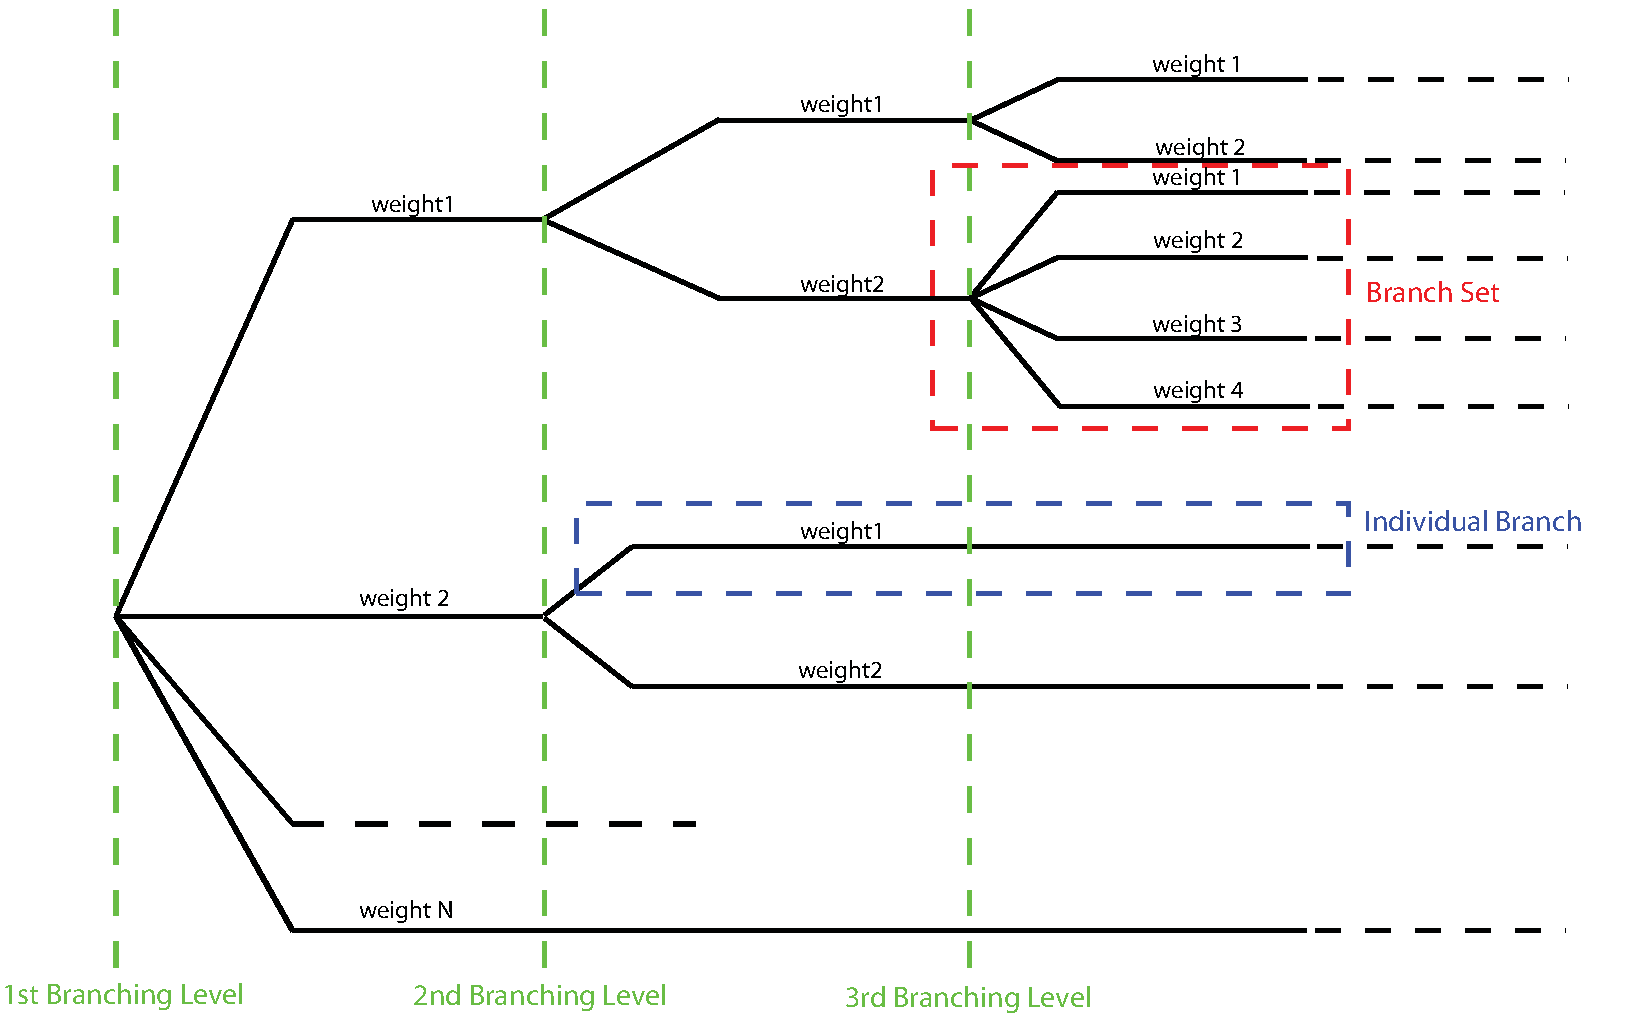
\includegraphics[width=15cm]{./figures/hazard/GenericLogicTreeStructure.pdf}
\caption{Generic Logic Tree structure as described in terms of branching 
levels, branch sets, and individual branches.}
\label{glts}
\end{figure}

\subsubsection{Logic trees as described in the nrml schema}
In the NRML schema, a logic tree structure is defined through the 
\Verb+logicTree+ element: 
%
\begin{Verbatim}[frame=single, commandchars=\\\{\}]
<\textcolor{red}{logicTree} logicTreeID="ID">
...
</\textcolor{red}{logicTree}>
\end{Verbatim}
%
A \Verb+logicTree+ contains as a sequence of \Verb+logicTreeBranchingLevel+ 
elements.
The position in the sequence of a \Verb+logicTreeBranchingLevel+ specifies 
the level of the tree where it is located. That is, the first 
\texttt{logicTreeBranchingLevel} element in the sequence represents 
the first level in the tree, the second element the second level in
the tree, and so on.
%
\begin{Verbatim}[frame=single, commandchars=\\\{\}]
<\textcolor{red}{logicTree} logicTreeID="ID">
	<\textcolor{green}{logicTreeBranchingLevel} branchingLevelID="ID_1">
		...
	</\textcolor{green}{logicTreeBranchingLevel}>
	<\textcolor{green}{logicTreeBranchingLevel} branchingLevelID="ID_2">
		...
	</\textcolor{green}{logicTreeBranchingLevel}>
	....
	<\textcolor{green}{logicTreeBranchingLevel} branchingLevelID="ID_N">
		...
	</\textcolor{green}{logicTreeBranchingLevel}>
</\textcolor{red}{logicTree}>
\end{Verbatim}
There are no restrictions on the number of tree levels that can 
be defined.

A \Verb+logicTreeBranchingLevel+ is defined as a sequence of 
\Verb+logicTreeBranchSet+ elements where each \Verb+logicTreeBranchSet+ 
defines a particular epistemic uncertainty inside a branching level. 

A branch set has two required attributes: \Verb+branchSetID+ and 
\Verb+uncertaintyType+. The latter defines the type of epistemic uncertainty 
this branch set is describing.
\begin{Verbatim}[frame=single, commandchars=\\\{\}]
<\textcolor{red}{logicTree} logicTreeID="ID">
...
	<\textcolor{green}{logicTreeBranchingLevel} branchingLevelID="ID_#">
		<\textcolor{blue}{logicTreeBranchSet} branchSetID="ID_1"
			uncertaintyType="UNCERTAINTY_TYPE">
			...
		</\textcolor{blue}{logicTreeBranchSet}>
		<\textcolor{blue}{logicTreeBranchSet} branchSetID="ID_2"
			uncertaintyType="UNCERTAINTY_TYPE">
			...
		</\textcolor{blue}{logicTreeBranchSet}>
		...
		<\textcolor{blue}{logicTreeBranchSet} branchSetID="ID_N"
			uncertaintyType="UNCERTAINTY_TYPE">
			...
		</\textcolor{blue}{logicTreeBranchSet}>
	</\textcolor{green}{logicTreeBranchingLevel}>
...
</\textcolor{red}{logicTree}>
\end{Verbatim}
Possible values for the \Verb+uncertaintyType+ attribute are:
\label{list_epistemic_unc}
\begin{itemize}
\item \Verb+gmpeModel+: indicates epistemic uncertainties on ground 
motion prediction equations
\item \Verb+sourceModel+: indicates epistemic uncertainties on source models
\item \Verb+maxMagGRRelative+: indicates relative (i.e. increments)
	epistemic uncertainties to be added (or subtracted, depending on 
	the sign of the increment) to the Guten\-berg-Richter maximum 
	magnitude value.
\item \Verb+bGRRelative+: indicates relative epistemic uncertainties 
	to be applied to the Guten\-berg-Richter b value.
\item \Verb+abGRAbsolute+: indicates absolute (i.e. values used to replace
 	original values) epistemic uncertainties on the 
	Guten\-berg-Richter a and b values.
\item \Verb+maxMagGRAbsolute+: indicates (absolute) epistemic 
	uncertainties on the Guten\-berg-Richter maximum magnitude.
\end{itemize}
There are no restrictions on the number of branch sets that can be defined 
inside a branching level.

A \Verb+branchSet+ is defined as a sequence of \Verb+logicTreeBranch+ 
elements, each specified by an \Verb+uncertaintyModel+ element (a string 
identifying an uncertainty mod\-el; the content of the string varies with
the \texttt{uncertaintyType} attribute value of the branchSet element) 
and the \texttt{uncertaintyWeight} element (specifying the probability/weight associated to the uncertaintyModel):
\begin{Verbatim}[frame=single, commandchars=\\\{\}]
<\textcolor{red}{logicTree} logicTreeID="ID">
...
	<\textcolor{green}{logicTreeBranchingLevel} branchingLevelID="ID_#">
		...
		<\textcolor{blue}{logicTreeBranchSet} branchSetID="ID_#"
				uncertaintyType="UNCERTAINTY_TYPE">
			<\textcolor{magenta}{logicTreeBranch} branchID="ID_1">
				<uncertaintyModel>
				UNCERTAINTY_MODEL
				</uncertaintyModel>
				<uncertaintyWeight>
				UNCERTAINTY_WEIGHT
				</uncertaintyWeight>
			</\textcolor{magenta}{logicTreeBranch}>
			...
			<\textcolor{magenta}{logicTreeBranch} branchID="ID_N">
				<uncertaintyModel>
				UNCERTAINTY_MODEL
				</uncertaintyModel>
				<uncertaintyWeight>
				UNCERTAINTY_WEIGHT
				</uncertaintyWeight>
			</\textcolor{magenta}{logicTreeBranch}>
		</\textcolor{blue}{logicTreeBranchSet}>
		...
	</\textcolor{green}{logicTreeBranchingLevel}>
...
</\textcolor{red}{logicTree}>
\end{Verbatim}
Depending on the \Verb+uncertaintyType+ the content of the 
\Verb+<uncertaintyModel>+ element changes:
\begin{itemize}
\item if \Verb+uncertaintyType="gmpeModel"+, the uncertainty model 
contains the name of a ground motion prediction equation (a list of 
available GMPEs are given in appendix A at page 
\pageref{sec:gmpes_list}), e.g.:
\begin{Verbatim}[frame=single, commandchars=\\\{\}]
<uncertaintyModel>GMPE_NAME</uncertaintyModel>
\end{Verbatim}
\item if \Verb+uncertaintyType="sourceModel"+, the uncertainty model contains 
the paths to a source model file, e.g.:
\begin{Verbatim}[frame=single, commandchars=\\\{\}]
<uncertaintyModel>SOURCE_MODEL_FILE_PATH</uncertaintyModel>
\end{Verbatim}
\item if \Verb+uncertaintyType="maxMagGRRelative"+, the uncertainty model 
contains the increment to be added (or subtracted, depending on the sign) 
to the Guten\-berg-Richter maximum magnitude:
\begin{Verbatim}[frame=single, commandchars=\\\{\}, samepage=true]
<uncertaintyModel>MAX_MAGNITUDE_INCREMENT</uncertaintyModel>
\end{Verbatim}
\item if \Verb+uncertaintyType="bGRRelative"+, the uncertainty model 
contains the increment to be added (or subtracted, depending on the 
sign) to the Guten\-berg-Richter b value:
\begin{Verbatim}[frame=single, commandchars=\\\{\}, samepage=true]
<uncertaintyModel>B_VALUE_INCREMENT</uncertaintyModel>
\end{Verbatim}
\item if \Verb+uncertaintyType="abGRAbsolute"+, the uncertainty model 
must contain one a and b pair:
\begin{Verbatim}[frame=single, commandchars=\\\{\}, samepage=true]
<uncertaintyModel>
A_VALUE B_VALUE
</uncertaintyModel>
\end{Verbatim}
    \item if \Verb+uncertaintyType="maxMagGRAbsolute"+, the uncertainty 
    model must contain one Guten\-berg-Richter maximum 
    magnitude value:
%
\begin{Verbatim}[frame=single, commandchars=\\\{\}, samepage=true]
<uncertaintyModel>
MAX_MAGNITUDE
</uncertaintyModel>
\end{Verbatim}
\end{itemize}
%
There are no restrictions on the number of \Verb+logicTreeBranch+ elements 
that can be defined in a \Verb+logicTreeBranchSet+, as long as the uncertainty 
weights sum to 1.0.

The \Verb+logicTreeBranchSet+ element offers also a number of optional 
attributes allowing for complex tree definitions:
\begin{itemize}
    \item \Verb+applyToBranches+: specifies to which \Verb+logicTreeBranch+ 
    elements (one or more), in the previous branching level, the branch set 
    is linked to. The linking is established by defining the IDs of the 
    branches to link to:
\begin{Verbatim}[frame=single, commandchars=\\\{\}, samepage=true]
applyToBranches="branchID1 branchID2 .... branchIDN"
\end{Verbatim}
    The default is the keyword ALL, which means that a branch set is by default 
    linked to all branches in the previous branching level. By specifying one or 
    more branches to which the branch set links to, non-symmetric logic trees 
    can be defined.
    \item \Verb+applyToSources+: specifies to which source in a source model 
        the uncertainty applies to. Sources are specified in terms of their IDs:
\begin{Verbatim}[frame=single, commandchars=\\\{\}, samepage=true]
applyToSources="srcID1 srcID2 .... srcIDN"
\end{Verbatim}
    \item \Verb+applyToSourceType+: specifies to which source type the 
    uncertainty applies to.  Only one source typology can be defined 
    (\Verb+area+, \Verb+point+, \texttt{simple\-Fault}, 
	\Verb+complexFault+), e.g.:
\begin{Verbatim}[frame=single, commandchars=\\\{\}, samepage=true]
applyToSources="area"
\end{Verbatim}
    \item \Verb+applyToTectonicRegionType+: specifies to which tectonic 
    region type the uncertainty applies to. Only one tectonic region type 
    can be defined (\texttt{Ac\-tive} \texttt{Shallow Crust}, 
    \Verb+Stable Shallow Crust+, \Verb+Subduction Interface+, 
    \texttt{Sub\-duc\-tion} \texttt{IntraSlab}, \texttt{Volcanic}), e.g.:
\begin{Verbatim}[frame=single, commandchars=\\\{\}]
applyToTectonicRegionType="Active Shallow Crust"
\end{Verbatim}
\end{itemize}
